% THIS IS SIGPROC-SP.TEX - VERSION 3.1
% WORKS WITH V3.2SP OF ACM_PROC_ARTICLE-SP.CLS
% APRIL 2009
%
% It is an example file showing how to use the 'acm_proc_article-sp.cls' V3.2SP
% LaTeX2e document class file for Conference Proceedings submissions.
% ----------------------------------------------------------------------------------------------------------------
% This .tex file (and associated .cls V3.2SP) *DOES NOT* produce:
%       1) The Permission Statement
%       2) The Conference (location) Info information
%       3) The Copyright Line with ACM data
%       4) Page numbering
% ----------------------------------------------------------------------------------------------------------------
% This .tex file (and associated .cls V2.4) produces:
%       1) The Permission Statement
%       2) The Conference (location) Info information
%       3) The Copyright Line with ACM data
%       4) NO page numbers
%
% ---------------------------------------------------------------------------------------------------------------
% It is an example which *does* use the .bib file (from which the .bbl file
% is produced).
% REMEMBER HOWEVER: After having produced the .bbl file,
% and prior to final submission,
% you need to 'insert'  your .bbl file into your source .tex file so as to provide
% ONE 'self-contained' source file.
%
% Questions regarding SIGS should be sent to
% Adrienne Griscti ---> griscti@acm.org
%
% Questions/suggestions regarding the guidelines, .tex and .cls files, etc. to
% Gerald Murray ---> murray@hq.acm.org
%
% For tracking purposes - this is V3.1SP - APRIL 2009

%\documentclass{acm_proc_article-sp}
\documentclass{sig-alternate}

\begin{document}

\title{Towards an adaptive middleware for\\ opportunistic environment: a mobile agent approach}

% You need the command \numberofauthors to handle the 'placement
% and alignment' of the authors beneath the title.
%
% For aesthetic reasons, we recommend 'three authors at a time'
% i.e. three 'name/affiliation blocks' be placed beneath the title.
%
% NOTE: You are NOT restricted in how many 'rows' of
% "name/affiliations" may appear. We just ask that you restrict
% the number of 'columns' to three.
%
% Because of the available 'opening page real-estate'
% we ask you to refrain from putting more than six authors
% (two rows with three columns) beneath the article title.
% More than six makes the first-page appear very cluttered indeed.
%
% Use the \alignauthor commands to handle the names
% and affiliations for an 'aesthetic maximum' of six authors.
% Add names, affiliations, addresses for
% the seventh etc. author(s) as the argument for the
% \additionalauthors command.
% These 'additional authors' will be output/set for you
% without further effort on your part as the last section in
% the body of your article BEFORE References or any Appendices.

\numberofauthors{3} %  in this sample file, there are a *total*
% of EIGHT authors. SIX appear on the 'first-page' (for formatting
% reasons) and the remaining two appear in the \additionalauthors section.
%
\author{
% You can go ahead and credit any number of authors here,
% e.g. one 'row of three' or two rows (consisting of one row of three
% and a second row of one, two or three).
%
% The command \alignauthor (no curly braces needed) should
% precede each author name, affiliation/snail-mail address and
% e-mail address. Additionally, tag each line of
% affiliation/address with \affaddr, and tag the
% e-mail address with \email.
%
% 1st. author
\alignauthor
Vinicius Pinheiro\\
       \affaddr{Department of Computer Science, University of S\~ao Paulo}\\
       \affaddr{Rua do Mat\~ao 1010, Cidade Universit\'aria}\\
       \affaddr{S\~ao Paulo, Brazil}\\
       \email{vinicius@ime.usp.br}
% 2nd. author
\alignauthor
Fabio Kon\\
       \affaddr{Department of Computer Science, University of S\~ao Paulo}\\
       \affaddr{Rua do Mat\~ao 1010, Cidade Universit\'aria}\\
       \affaddr{S\~ao Paulo, Brazil}\\
       \email{kon@ime.usp.br}
% 3rd. author
\alignauthor 
Alfredo Goldman\\
       \affaddr{Department of Computer Science, University of S\~ao Paulo}\\
       \affaddr{Rua do Mat\~ao 1010, Cidade Universit\'aria}\\
       \affaddr{S\~ao Paulo, Brazil}\\
       \email{gold@ime.usp.br}
}
% There's nothing stopping you putting the seventh, eighth, etc.
% author on the opening page (as the 'third row') but we ask,
% for aesthetic reasons that you place these 'additional authors'
% in the \additional authors block, viz.
\date{01 october 2009}
% Just remember to make sure that the TOTAL number of authors
% is the number that will appear on the first page PLUS the
% number that will appear in the \additionalauthors section.

\maketitle
\begin{abstract}

The mobile agent paradigm has emerged as a promising alternative to overcome
the construction challenges of opportunistic grid environments.
This model can be used to implement mechanisms that enable
application execution progress even in the presence of failures, such as
those presented by the MAG middleware (Mobile Agents for Grids). 
MAG includes retrying, replication, and checkpointing as
fault-tolerance techniques; they operate independently from
each other and are not capable of detecting changes on resource availability.
In this paper, we describe a MAG extension that is capable of migrating agents when 
nodes fail, that optimizes application progress by keeping only the most advanced 
checkpoint, and that migrates slow replicas.

\end{abstract}

% A category with the (minimum) three required fields
\category{C.2.4}{Distributed Systems}{Distributed Applications}

\terms{Experimentation}

\section{Introduction}

Opportunistic grids are distributed environments built to leverage the
computational power of idle resources geographically spread across different
administrative domains. These environments comprise many characteristics such as
high level of heterogeneity and large changes on resource availability. 

In distributed systems such as opportunistic grids, failures can occur due to
several factors, most of them related to resource heterogeneity and
distribution. These failures together with the resource usage by its
owners modify grid resource availability (i.e.,
resources can be active, busy, offline, crashed, etc.). The middleware should
be able to monitor and detect such changes, rescheduling 
applications across the available resources and dynamically tuning the fault
tolerance mechanisms to better adapt to the execution environment. 

In this work, we implemented dynamic fault tolerance mechanisms for grid
applications. These mechanisms compose a feedback control system
\cite{steere99, goel99}, gathering and analyzing information about the execution
progress and adjusting its behavior accordingly. To build these mechanisms we
rely in the mobile agent paradigm~\cite{pham98}. Mobile agents are programs that can move
from one resource to another in an autonomous way, carrying its data and
execution state, resuming its execution at the destination. We argue that
agents are suitable for constructing opportunistic grids due to intrinsic agent characteristics, 
such as:

\begin{enumerate}
    \item \emph{Cooperation}: agents have the ability to interact and cooperate
    with other agents; this can be explored for the development of complex
    communication mechanisms among distributed application tasks.
   
    \item \emph{Autonomy}: agents are autonomous entities, meaning that their
    execution goes on without any or with little intervention from the clients
    that started them. This is a suitable model for submission and execution
    of grid applications.
  
    \item \emph{Heterogeneity}: most mobile agent platforms can be executed
    in heterogeneous environments, an important characteristic for better use
    of computational resources across multi-organization environments.
  
    \item \emph{Reactivity}: agents can react to external events, such as
    variations on resources availability.
  
    \item \emph{Mobility}: agents can migrate from one node to another,
    moving part of the computation being executed, helping to balance the load on grid nodes.
\end{enumerate}

Since 2004, our research group has been using the agent paradigm
for developing a grid software infrastructure, leading to the MobiGrid \cite{barbosa04} and MAG \cite{lopes05}
projects  that are based on the
InteGrade middleware \cite{goldchleger04}, which follows an opportunistic approach, where
workstations idle computing power is used for executing
computationally-intensive parallel applications.

This work describes enhancements to the MAG middleware that
address the high dynamism of opportunistic
grids, managing effectively execution and resource allocation for both sequential and
parametric applications. 

In the next section, we present some of the related work. In
Section~\ref{sec:arch}, we present the MAG architecture and its fault tolerance
mechanisms. In Section~\ref{sec:adapt}, we describe the implementation
of the dynamic replication and unified checkpointing mechanisms. We describe
simulation results that assess our proposal in Section~\ref{sec:eval}.
Finally, in the last section, we present our conclusions and future work.

%============================================================================

\section{Related Work}

There are several works that are related to this paper, some related to the
systems giving support for parametric applications, some related to
running long sequential applications on non-dedicated environments, and finally
some works are related to the use of mobile agents on grid middleware.

The most well known work was provided by research on extraterrestrial life on
the SETI program~\cite{seti} where more attention were paid on security aspects
and on the reliability of the results. More recently, the BOINC
project~\cite{boinc} proposed an infrastructure allowing the execution of
different programs which can be executed on volunteer computers spread around
the world. There exist similar projects both with a fixed algorithm as
Mersenne~\cite{mersenne}, and where different algorithms or challenges can be
programmed~\cite{distributed}. However, on these projects the support for long
running sequential applications is mostly restricted to local checkpoints (with
few exception like~\cite{climate}, or the use of replication to guarantee the
progress of the individual applications). Another bag-of-tasks approach is
based on OurGrid~\cite{cirne06}, however the main focus is on dealing with
the middleware infrastructure and not on the individual sequential
applications.

Several works deals with checkpointing techniques to guarantee the progress of
sequential long running applications. One that is directly related to our
work is the Grid-WFS framework~\cite{hwang03}. In this work the authors studied several approaches to
deal with failures on machines. The handling techniques were: retrying, checkpointing,
replication, and replication with checkpointing. They concluded that in grid
environments with high down-time, as it can happen in opportunistic environments,
the replication with checkpointing outperforms the other ones, using as comparison
the lower completion time. The Condor project also provides some fault tolerance mechanisms
to deal with instable and opportunistic environments: checkpointing and process
migration. However, Condor does not perform task replication which would be
used to improve application execution progress in the presence of host and
network failures.

Several works present the use of mobile agents on grid environments, some using
opportunistic contexts (e.g. UWAgents~\cite{fukuda06}), but most of them
presents characteristics more related to the middleware, not the application
(e.g. ARMS~\cite{cao02} and the works published by Loke~\cite{loke03} and
Martino and Rana~\cite{martino04}). Some of the mobile agent work were done
within our project InteGrade~\cite{goldchleger04}. The first ideas on using
mobile agents on an opportunistic grid appeared in~\cite{barbosa04} where an
architecture based on Aglets~\cite{aglets} is first presented, and then
evaluated with the use of several replicas in~\cite{barbosa05}. More recently a
work based on the mobile agents framework Jade~\cite{jade} was also
presented~\cite{lopes05,lopes06_2}, where there is application instrumentation,
to provide transparent checkpointing and some work on fault tolerance.

To the best of our knowledge this paper is the first one that specifically uses
mobile agents combined with replication and checkpointing techniques, within a
grid middleware, to provide dynamic fault tolerance mechanisms for sequential
and parametric applications on opportunistic environments.

%===========================================================================e

\section{The middleware InteGrade/MAG}\label{sec:arch}

The InteGrade project involves the development of a grid middleware that
leverages the idle computational power of desktop machines. 
Its architecture follows a hierarchy in which each node can assume
different responsibilities. The Cluster Manager is represented by one or more
nodes that are responsible for managing that cluster and performing
communication with other clusters. A Resource Provider node is the one that
exports part of its resources, making them available to grid users. A User Node
is one belonging to a grid user who submits grid applications. As we can see in
Figure \ref{fig:integrade}, the InteGrade architecture follows a two-tier
intra-cluster hierarchy combined with a inter-cluster network.

\begin{figure}[th]
\centering 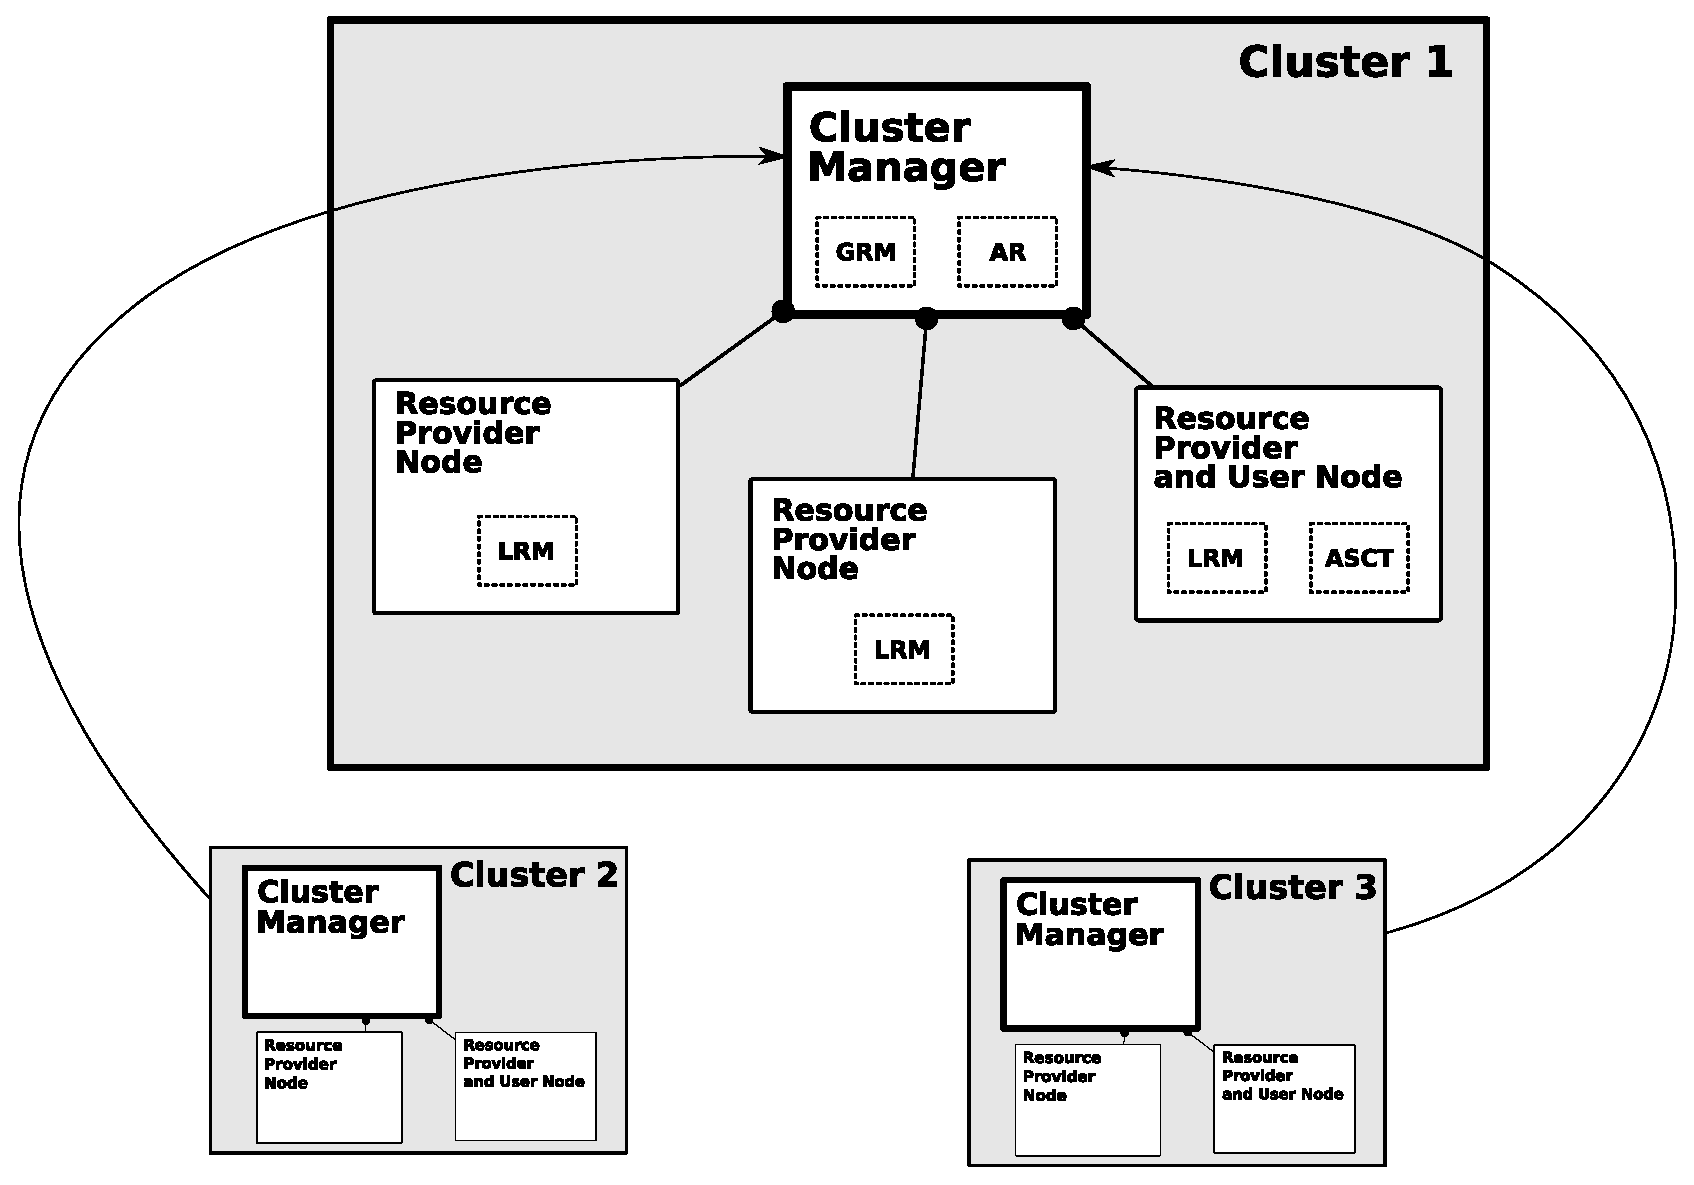
\includegraphics[width=1\columnwidth]{images/integrade2_ieee.eps}
\caption{InteGrade architecture}
\label{fig:integrade}
\end{figure}

The MAG project \cite{lopes05} introduces the mobile agent technology as a new way
of executing applications on InteGrade. Through MAG, the grid user can submit
Java applications, not previously supported by the native InteGrade middleware. This is
performed by dynamically loading sequential grid applications into mobile
agents. MAG uses JADE (\emph{Java Agent Development Framework}) ~\cite{jade} as the agent
platform to provide agent services such as communication and life cycle
monitoring. 
To avoid duplication of efforts, the MAG project was built on top of
some InteGrade components: Global Resource Manager (GRM), Local Resource
Manager (LRM), Application Repository (AR) and Application Submission and
Control Tool (ASCT) (see Figure \ref{fig:integrade}). 
The GRM is the main grid component and is executed
in the Cluster Manager Nodes; it holds information about the registered
LRMs and is able to dispatch tasks to them. The LRM is executed in
each Resource Provider node; it loads the execution environment and
executes tasks submitted to them. The AR provides a cluster repository to
store application binaries. Finally, the ASCT provides a user interface for grid application submission,  
monitoring, and collection of computation results.

In addition, the MAG architecture also adds components that provides
mobile agents capabilities and fault-tolerance mechanisms:

\begin{enumerate}

    \item The \emph{ExecutionManagementAgent (EMA)}  stores
    information about current and past executions, such as current execution state
    (accepted, running, finished), input arguments, and scheduled machines. This information
    can be retrieved to restore applications to the point in which they were before
    the failure.

    \item The \emph{AgentHandler} runs on top of the LRMs and 
    works as a proxy to the JADE agent platform, instantiating
    MAGAgents for each requested execution.

    \item The \emph{ClusterReplicationManagerAgent (CRM)} receives requests
    for execution with replicas from the GRM and creates an ERM agent to handle the request.

    \item The \emph{ExecutionReplicationManagerAgent (ERM)} distributes the replicas across the 
    LRMs in the distributed system.

    \item The \emph{StableStorage} agent receives the compressed
    checkpoints, storing them in the file system and retrieving them when
    prompted. This agent runs in the Cluster Manager node.

    \item The \emph{MAGAgent} is the MAG main component; it
    wraps the application, instantiates it, and catches its exceptions. It also controls application 
    life cycle.

    \item The \emph{AgentRecover} is created on demand by the MAGAgents  to recover
    execution in the presence failures.

\end{enumerate}

\subsection{Fault-tolerance in MAG\label{sec:faulttolerance}}

The MAG fault-tolerance mechanisms can be combined to meet different scenarios of resource
availability, resulting in 4 different strategies:

\begin{enumerate}
    \item \emph{Retrying}: every time the application fails (by throwing an exception), its agent migrates to another node.

    \item \emph{Replication}: multiple application replicas are submitted
for execution at the same time. When one of the replicas finishes, the others
are discarded to avoid waste of resources. In case of failure,
retrying is applied.
   
    \item \emph{Checkpointing}: the application periodically saves its execution
state in a stable storage. In case of application failure, retrying is
applied, but the execution is resumed from the most recent checkpoint.
 
    \item \emph{Checkpointing with Replication}: each replica periodically saves
its execution state in a stable storage. Retrying and resuming of execution is
applied independently for each replica in the presence of failures.

\end{enumerate}

Currently, the MAG middleware supports only the submission of parametric (bag-of-tasks) and
sequential Java applications. This is implemented by extending
the {\tt MagApplication} class, wrapping the application code into a mobile agent and submitting
it to the agent platform. 

In the MAG middleware, the checkpoint mechanism is obtained through code
instrumentation provided by the \emph{MAG/Brakes} framework~\cite{brakes00}.

\section{Improving MAG: towards an adaptive middleware}\label{sec:adapt}

As shown in Section \ref{sec:faulttolerance}, the MAG middleware supports
multiple fault-tolerance techniques, but these techniques operate solely.
Besides, they do not perform any automatic adjustments to adapt themselves
to changes in resource availability. If a machine is turned off, for
example, all the replicas that were executing on it are lost as MAG only
detects failures at the application layer. These replicas are not replaced and
the middleware does not make use of their checkpoints.

Events such as network partitioning, crash failures, machine shutdowns,
nodes joining the grid, and nodes leaving the grid, define the resource
availability of the executing environment. Thus it is desirable that the middleware 
include fault-tolerance mechanisms to adapt dynamically to these changes.

\subsection{Unified Checkpoint}

As explained previously, the MAG fault-tolerance mechanisms work
independently from each other. This model does not scale well since it
makes all replicas perform checkpointing periodically. 
This increases the communication traffic between resource provider nodes and
the stable storage, consuming more grid resources. 
Another disadvantage of this model is related to resource
heterogeneity: in a heterogeneous environment like opportunistic grids some
replicas will advance its execution faster than the others. If the most
advanced replica crashes in a way that MAG cannot detect, its latest checkpoint
will not be used by the slower replicas and part of the execution will be
lost. 

\begin{figure}[th]
\centering 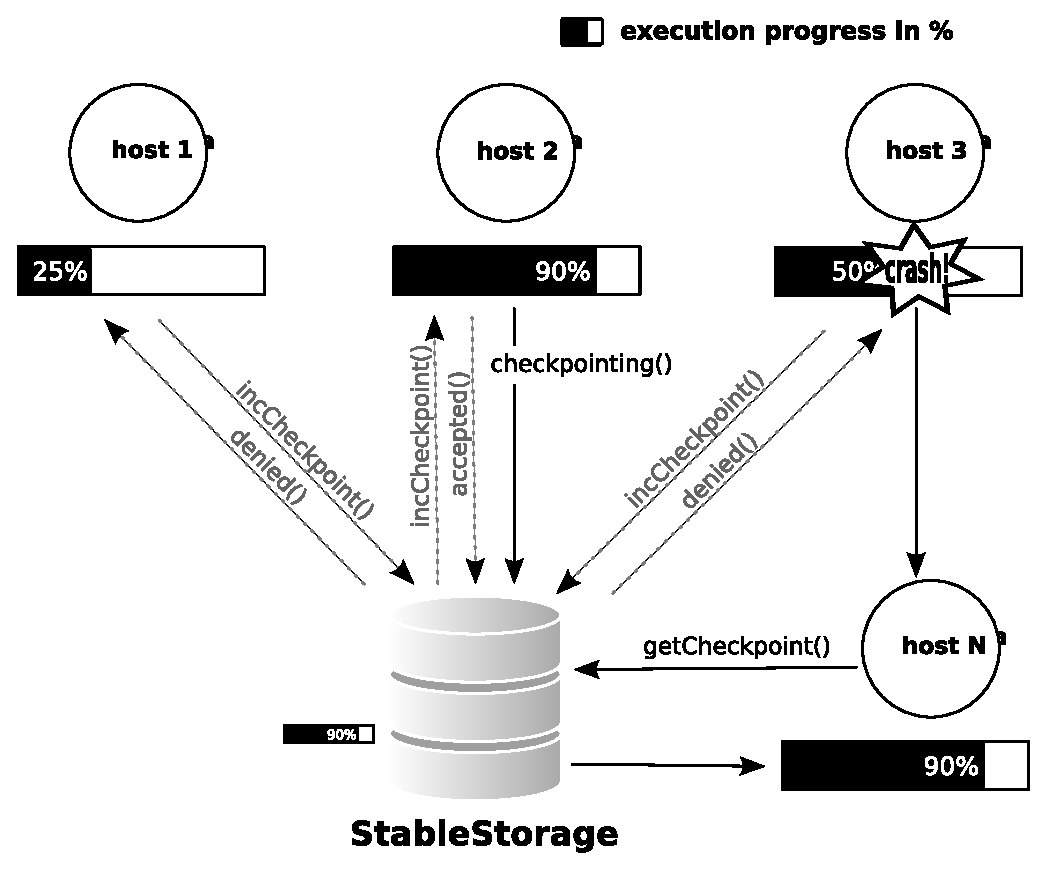
\includegraphics[width=0.9\columnwidth]{repCheckNovoFalha.eps}
\caption{Unified Checkpoint model}
\label{fig:repCheckNovo}
\end{figure}

To resolve this problem, we propose a mechanism named Unified Checkpoint. In
this new model, the replicas periodically send information about their
execution progress and only the most advanced replica is authorized to perform
checkpointing. To enable this feature, the applications must invoke a method
which increases a counter. It is in charge of the application programmer to
choose the most appropriate places to put these invocations into the code
since this is a very application-specific issue. When the replica hits a
checkpoint, it sends only the value of the counter and the Stable Storage
compares this value to the ones sent by the other replicas. Only the
replica with the highest counter value will be requested to save the
checkpoint. This model is depicted in Figure \ref{fig:repCheckNovo}.

In Figure \ref{fig:repCheckNovo}, the replica running on host 2 is the most advanced one. When
the replica running on host 3 crashes, the MAG recovery mechanism is executed
and a new replica is created on host N and the Stable Storage is queried for the
checkpoint. The checkpoint stored by the most advanced replica is the only
option and so it is sent to the new replica, which resumes its execution
from this advanced stage. 

\subsection{Replica Replacement}

Although the checkpointing and the replication of tasks now operate together to
form a more integrated fault tolerance system, some events, such as machine crashes,
may reduce the number of replicas in execution. Besides,
it would be interesting to compare the replica counters to
detect replicas that are slow and decide whether they should be moved 
to another, hopefully faster, computing node

To accomplish that, we propose a feedback control system based on periodical
analysis of resource availability. This system is depicted in Figure
\ref{fig:feedback}.

\begin{figure}[th]
\centering 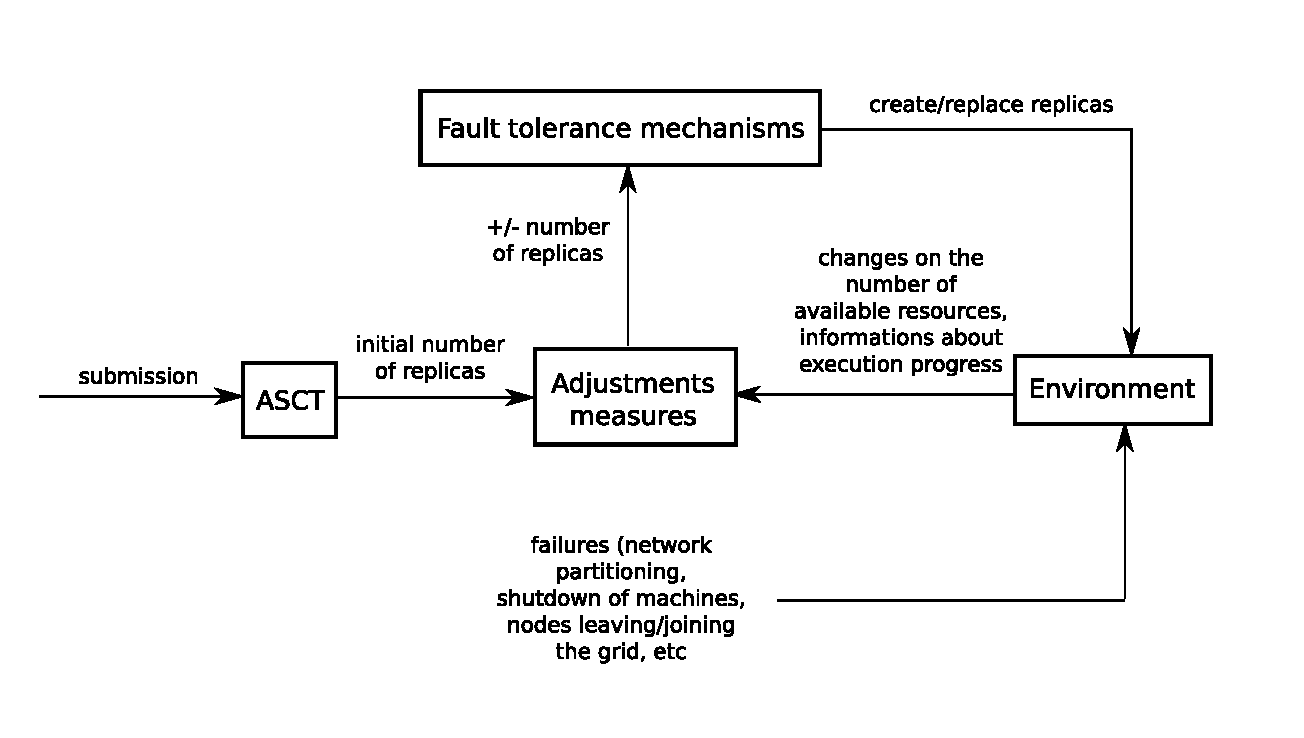
\includegraphics[width=1.1\columnwidth]{feedback.eps}
\caption{Dynamic replication: a feedback system model}
\label{fig:feedback}
\end{figure}
%
Initially, the grid user submits an application to the grid. The application
replicas are created and submitted for execution on the grid nodes. The number of
replicas created will be equal to a fixed number defined by the user, but
respecting a maximum value of replicas for each application\footnote{The
maximum number of replicas allowed can be customized by grid
administrators}. While running, these replicas are susceptible to failures
related to intrinsic characteristics of opportunistic environments such as
network partitions, machine shutdown, out-of-memory errors, etc. These
failures reduce the number of replicas in execution and also modify the number
of available resources. These changes are detected by the system that, after a
period without getting responses from the crashed/offline nodes, updates the
list of nodes that are still alive (and the new ones that have joined or
rejoined the grid recently). Furthermore, during this time, some
replicas may become delayed. Based on this information, new replicas are
created and late ones are migrated to the new nodes. 
The Unified Checkpoint will be present throughout this process, so new replicas will resume its execution
from the checkpoint of the most advanced replica. This mechanism works even
when the most advanced replica crashes, as its last checkpoint remains stored
at the Stable Storage so that the new replica can resume from it.

In the current version, the Stable Storage is a single point of failure for our
system. This problem could be solve in the future by using the Jade agent
replication mechanism to implement redundancy in the checkpoint storage.

\section{Experiments and simulations}\label{sec:eval}

In this section, we present an event-based simulation in various scenarios,
demonstrating the potential value of adding dynamic fault-tolerance mechanisms
to MAG. Our analysis focuses on task execution times and resources consumption.
To run our simulation scenarios, we use the GridSim toolkit~\cite{buyya02}. The
parameters used in our simulation (mostly borrowed from \cite{plank98,
beguelin97}) follow. 

\begin{itemize}
    \item \emph{Failure rate ($\lambda$)} is a random variable
representing an arrival rate of failures governed by a Poisson distribution.
TBF (time between two adjacent failures) is a random variable governed by an
exponential distribution with MTBF representing the mean;
    
    \item \emph{Downtime (D)} is the average time following a failure of a
task before it is up again, governed by an exponential distribution.
   
    \item \emph{Number of replicas (N)} is the number of copies of an
application, with each running on different machines.  
\end{itemize}

We simulate a cluster environment with 100 heterogeneous machines connected by
a 100Mbps network. The processing power of the resources were generated
randomly from 800 to 1600 based on the SPECfp benchmark~\cite{spec06}.

We used 3 parameters to model the tasks: number of instructions in MI (millions
of instructions), binary size (in bytes) and output file size (in bytes). In
our experiments we choose to simulate long running tasks and, to do so, each
task submitted has 604800000 MI, the binary size is 320 Kilobytes and the
output file size is 15,6 Kilobytes. If we consider the most powerful machine
allowed in our experiments, it would take 105 hours to execute the task.

We measured the task execution times to compare the performance of the proposed
techniques against the old model. We used 2, 4, 8, and 16 replicas and fixed 60
minutes as the MTBF value to obtain a $\lambda$ of 24 failures per day. The
average downtime was fixed to 30 minutes. These values were used to simulate a
very inhospitable environment to distributed processing like student
laboratories, where machines are regularly turned off and rebooted. For each
number of replicas, we performed 40 simulations, measuring task execution
times, computing the arithmetic mean and the 95\% confidence interval with a
t-Student distribution. We assumed that the application execution time is the
execution time of the replica that finishes first. The results are plotted in
Figure \ref{fig:adapt-mag}.

\begin{figure}[th]
\centering 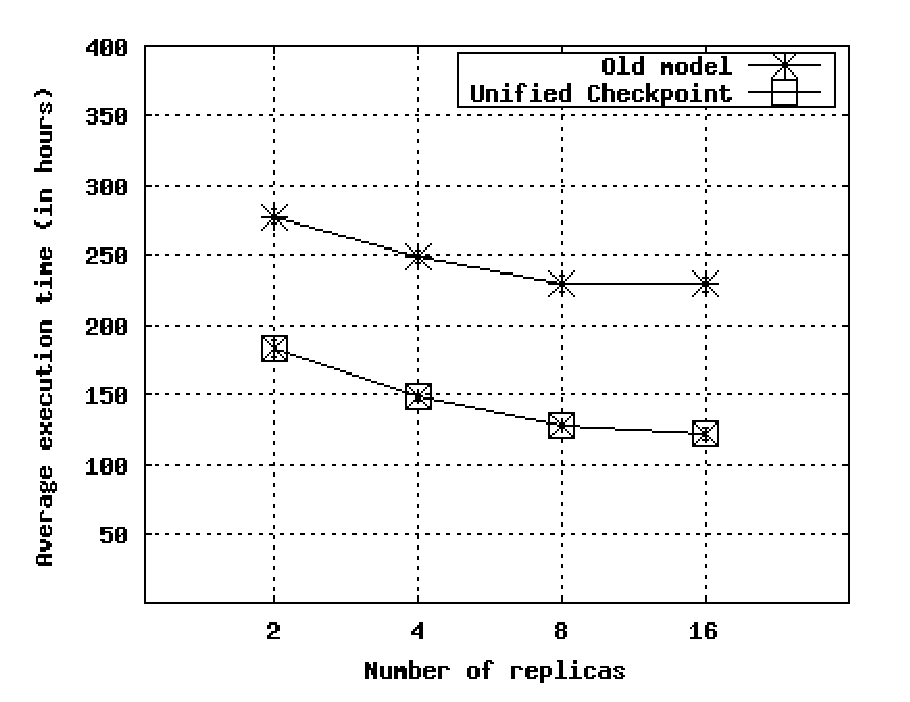
\includegraphics[width=1.1\columnwidth]{49-55_scenario.eps}
\caption{Performance comparison: Unified Checkpoint versus old model}
\label{fig:adapt-mag}
\end{figure}

First of all, it becomes clear that increasing the number of replicas results
in shorter execution times in both strategies. But we can see a considerable
gain in the total execution time when using the dynamic strategy presented in
this paper. The potential advantage of adopting the Unified Checkpoint
mechanism occurs independently of the number of replicas used in our
simulation. In all cases, the Unified Checkpoint outperforms the old model
obtaining better execution times (at least 34\% lower). This difference
increases as the number of replicas increases, achieving its maximum
performance improvement when 16 replicas were submitted (execution time 47\%
lower).  In the simulated scenarios, which are common in the field of
High-Performance Computing, the amount of time saved when using the Unified
Checkpoint varied between 95 and 107 hours.


\section{Conclusions}

Grid middleware hides the complexity related to distribution and
heterogeneity and must efficiently address issues such as management
and allocation of distributed resources, dynamic task scheduling, fault
tolerance, support for high scalability and great heterogeneity of software and
hardware components, protection, and security. 

The mobile agents paradigm are suitable for dealing with the complexity
of building the grid software infrastructure due to its intrinsic
characteristics, such as cooperation, autonomy, heterogeneity, reactivity, and
mobility. In this work, we present the Unified Checkpoint
mechanism, which combines dynamic task replication, replica substitution, and
checkpointing to provide fault tolerance for sequential and parametric
applications. We use the MAG middleware as the basis for implementing these
mechanism. This middleware benefits from the mobile agent paradigm to
encapsulate the applications submitted to the grid. 

We demonstrated through our experiments that, in opportunistic environments,
it is crucial to support dynamic fault tolerance mechanisms to
achieve high performance as well as to make a better use of the available
resources in a highly heterogeneous and unstable environment.

Currently, we are investigating other self-optimization and adaptive mechanisms
to add to our feedback system. We are currently measuring the benefits of increasing
or decreasing the number of replicas dynamically according to three factors: failure rate
of the execution environment, number of free resources, and amount of tasks to
be scheduled. We are also investigating the impact of changing the
checkpointing interval according to the failure rate and the size of the
checkpoints to optimize application completion time. 

%\end{document}  % This is where a 'short' article might terminate

% The following two commands are all you need in the
% initial runs of your .tex file to
% produce the bibliography for the citations in your paper.
\bibliographystyle{abbrv}
\bibliography{bibliografia}  % sigproc.bib is the name of the Bibliography in this case
% You must have a proper ".bib" file
%  and remember to run:
% latex bibtex latex latex
% to resolve all references
%
% ACM needs 'a single self-contained file'!
%
\balancecolumns
% That's all folks!
\end{document}
